\documentclass[epsfig]{article}
\usepackage{epsfig}
\usepackage{amsmath}
\usepackage{verbatim}
\usepackage{booktabs}
\usepackage{subfig}
\usepackage{diagbox} 
\usepackage{graphicx}
\usepackage[english]{babel}
\usepackage{float}
\textwidth 6.7in
\oddsidemargin -0.1in
\textheight 8.50in
\topmargin -0.55in
\renewcommand{\textfraction}{0.25}
\renewcommand{\floatpagefraction}{0.7}
\markboth{}{\sl E. Mer\'enyi \hfil COMP / ELEC / STAT 502 \hfil Homework 4 }
\pagestyle{myheadings}
\def\bpar{\vskip26pt}
\def\npar{\vskip13pt}
\def\spar{\vskip10pt}
\begin{document}
\parindent=0pt
\null
{\bf 
\npar
Zhuo Chen, Yidan Pan

Equally contributed
\bpar
}


{\bf \centering
	\npar
	Homework 4
	\bpar
}


{\bf 
	\npar
Problem 2
	\bpar
}


{\bf 
	\npar
	a Report network parameters
	\bpar
}

\begin{table}[htbp] 
	\center
	\caption{Parameters of Training BP Network to Fit $f(x) = 1/x$}
	\label{tab:NP}
	%\scalebox{0.9}{ % You can scale the size of the table by changing this number
	\scalebox{1.0}{
		\begin{tabular}{p{4cm} p{.05cm} p{8cm}}
			\toprule
			\multicolumn{3}{l}{\bf Network parameters} \\
			\bottomrule \noalign{\smallskip}
			Topology & & $(1 + 1_{Bias})$ --- $10$ --- $1$ \\
			Transfer function & & tanh with slope of 1 \\
			\toprule
			\multicolumn{3}{l}{\bf Learning parameters} \\
			\bottomrule \noalign{\smallskip}
			Initial weights & & drawn from U[-0.1, 0.1] \\
			Learning rate ($\alpha$) & & 0.01 \\
			Momentum & & none\\
			Epoch size ($Epoch$)& &  200 \\
			Stopping criteria & &  error ($Err_{RMSD}$) $ \le 0.05 $ OR  learn count (t) $ > 4,000,000 $\\
			Error measure($Err_{RMSD}$) & &  Square root of the sum of $(D-y)^2$ that averaged over all training or testing samples (see formula (1) below)\\\toprule
			\multicolumn{3}{l}{\bf Input / output data, representation, scaling} \\
			\bottomrule \noalign{\smallskip}
			\# training samples ($N_{tr}$)& & 200 (x values drawn randomly from U[0.1,1])\\
			\# test samples ($N_{tst}$)& & 100 (x values drawn randomly from U[0.1,1])\\
			Scaling of inputs & &  no scaling \\
			Scaling of outputs & &  map [global min, global max] to [-1,1] \\
			
			\bottomrule \noalign{\smallskip}
			
		\end{tabular}
	} % end scalebox
\end{table}

The formula of the error we computed is:

$$(1)\ \ \ Err_{RMSD}= \sqrt{{1\over{|X|}}\sum_{k=1}^{|X|}(D^k-y^k)^2}$$

Where $k$ is the sample index, $X$ is either the whole training or testing data set at a particular learn count. Based on the parameter we used, The size of $X$ is constant: 200 for training set, 100 for testing set.
\spar
\spar
\spar
\spar
{\bf 
	\npar
	c Plot performance indicator of the network
	\bpar
}
We use $Err_{RMSD}$(RMSE) as the performance indicator. The formula is shown as above. The figure shows the RMSE of training set. The RMSE is calculated every 10000 steps(50x200, where 200 is the size of training input set). We saw that  two spikes appeared in the process.

\begin{figure}[!htb] 
	\centering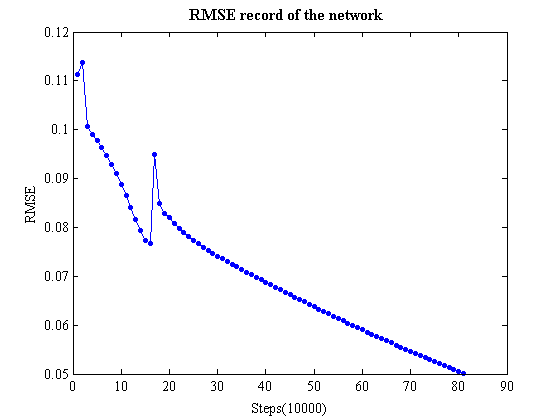
\includegraphics[width=4.5in]{fig1.png} 
\end{figure} 

\spar

After that, we compared the actual output with desired output after training is finished. The data is shown in the figure below:

\begin{figure}[!htb] 
	\centering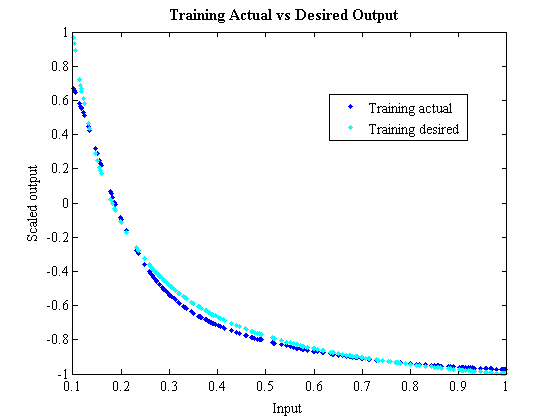
\includegraphics[width=4in]{fig2.png} 
\end{figure} 



The desired output vs actual output. The actual output is shown in blue and the desired output is shown in  In this run, 812400 steps were taken to make the final RMSE not higher than 0.05 (the average error we accept is 2.5\%).

{\bf 
	\npar
	d Number of learning step
	\bpar
}

We set the criteria as RMSE $\le$ 0.05 or number of step exceeds 4,000,000. After running the script using the parameters given above for 20 times, the average steps for achieving RMSE $\le$ 0.05 is 756620, while the standard deviation is 203769. Though the minimum required step is good, further optimization on the parameters is required to generate a more stable learning network.
\spar

{\bf 
	\npar
	e Training accuracy
	\bpar
}
The figure showed below compared the RMSE of test set and training set per each 10000 steps (50x200, where 200 is the size of training input set). The RMSE of testing set are shown in red, and the RMSE of training set are shown in blue. The RMSEs of test set in large step number are even lower than the training set.

It is one thing that need to be highlighted that there are actually 50 training runs interval between each point in the figure. For training set, each run goes through 200 samples, and these will be 10000 steps. For test set, each run goes through 100 samples, and these will be 5000 steps. 
\spar
{\bf Note: The definition of steps in batch learning should be different from online learning. Though we were using batch learning, here we kept using the definition of online learning (which made the count of steps a huge number).} 

\begin{figure}[!htb] 
	\centering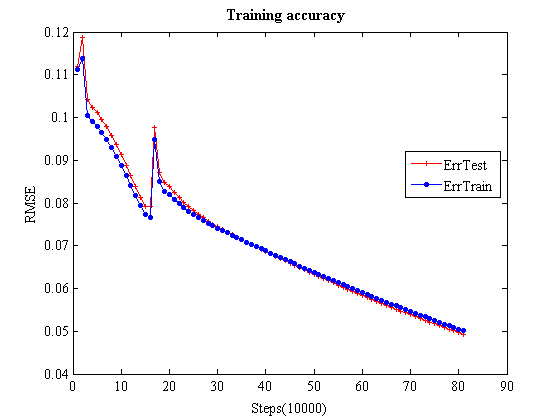
\includegraphics[width=4.5in]{fig3.png} 
\end{figure} 

After training is finished, the actual vs desired output for all points of both the training and testing data set is shown in the figure below:

\begin{figure}[!htb] 
	\centering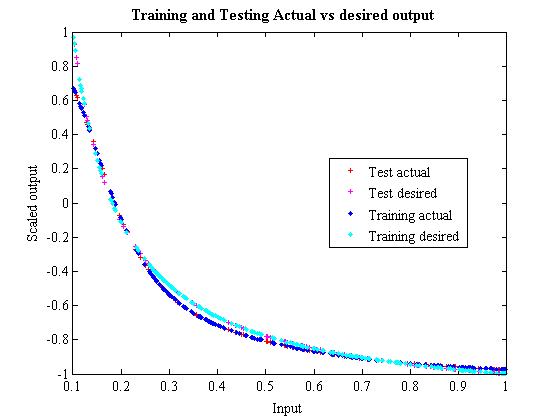
\includegraphics[width=4.5in]{fig4.png} 
\end{figure} 

It is clear that the two curves formed by the actual outputs coincide, though the points do not coincide in general. The same pattern is shown in the two curves formed by the desired outputs of training set and testing set. This data indicates that the recall ability of this net work is pretty good.

{\bf 
	\npar
	f Increasing the steps
	\bpar
}

We also tried to increase the number of steps. During training for 20,000 cycles, the changing of RMSE of both training set and test set are shown in the figure below:

\begin{figure}[!htb] 
	\centering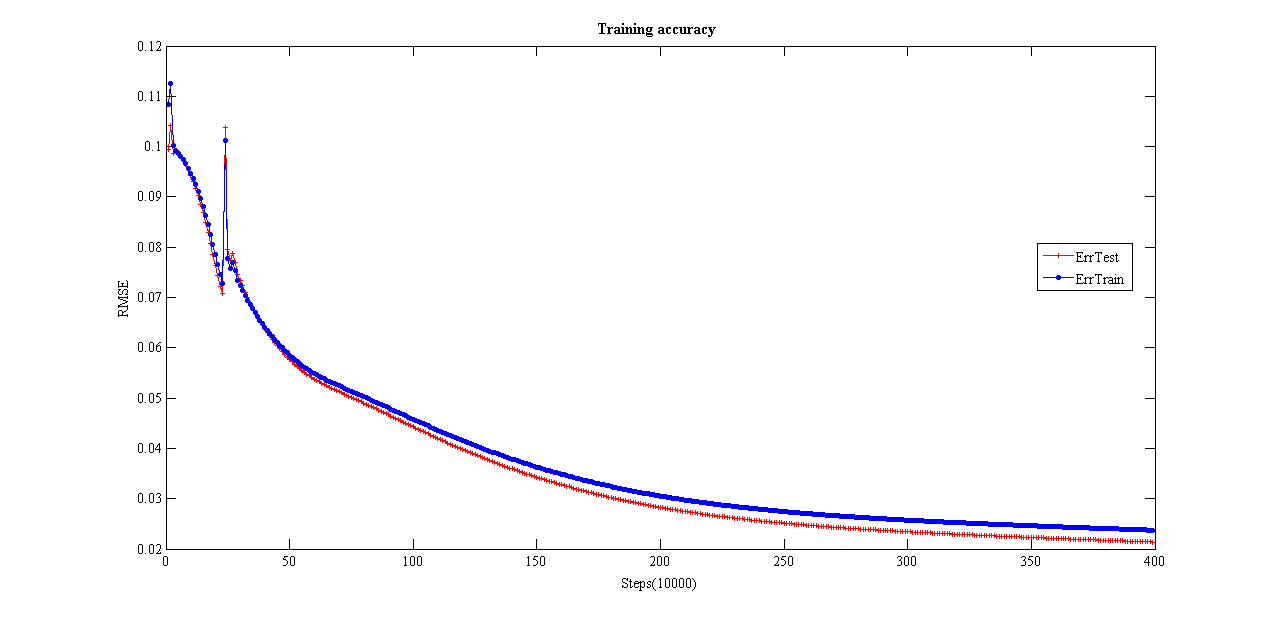
\includegraphics[width=6in]{fig5.png} 
\end{figure} 

The final RMSE of testing set is 0.0214, and the final RMSE of training set is 0.0237. We tried multiple times, and all the trends are similar: we saw some spikes at the very beginning, and then the error rate decreases and becomes flat.
\spar
The figure below compared the output pair of testing set and training set. From this we can see that while the general pattern are similar, the fitting is better than the one we performed above.
\begin{figure}[!htb] 
	\centering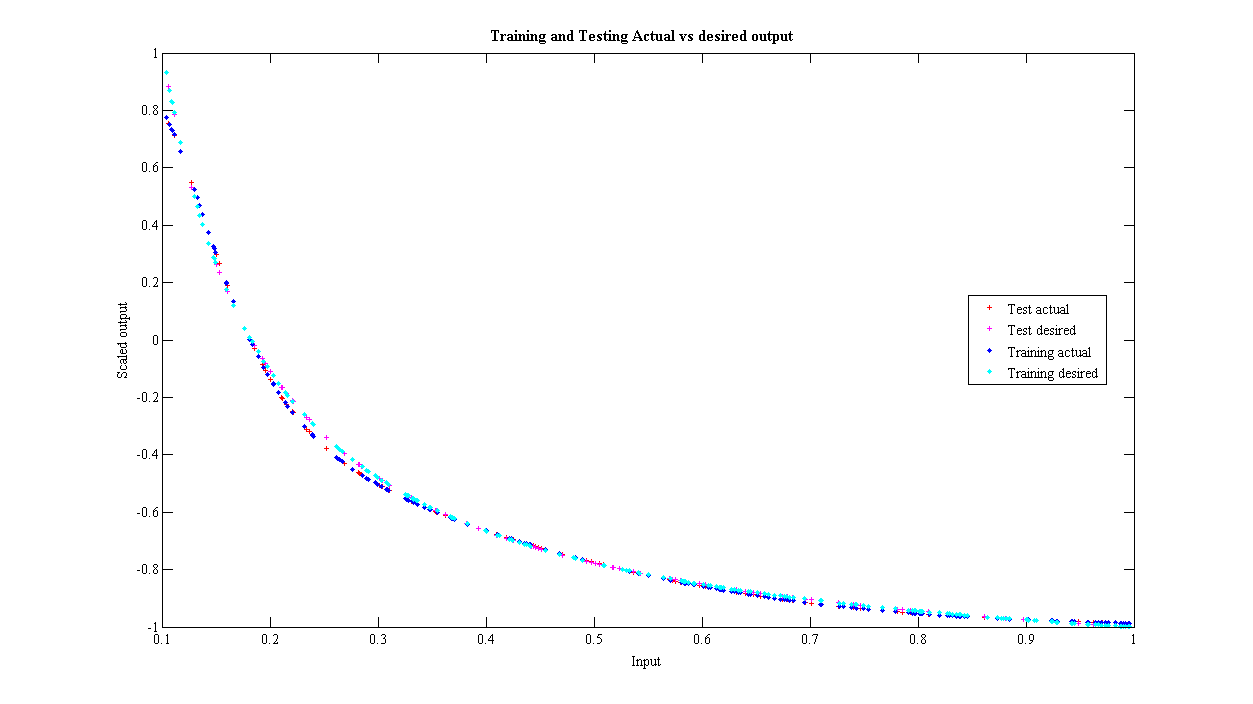
\includegraphics[width=6in]{fig6.png} 
\end{figure} 

{\bf 
	\npar
	Problem 3
	\bpar
}


\begin{table}[htbp] 
	\center
	\caption{General parameters of Training BP Network to Fit $f(x) = 1/x$}

	%\scalebox{0.9}{ % You can scale the size of the table by changing this number
	\scalebox{1.0}{
		\begin{tabular}{p{4cm} p{.05cm} p{8cm}}
			\toprule
			\multicolumn{3}{l}{\bf Network parameters} \\
			\bottomrule \noalign{\smallskip}
			Topology & & $(1 + 1_{Bias})$ --- Varies, refer to the table in each part of the answer --- $1$ \\
			Transfer function & & tanh with slope of 1 \\
			\toprule
			\multicolumn{3}{l}{\bf Learning parameters} \\
			\bottomrule \noalign{\smallskip}
			Initial weights & & drawn from U[-0.1, 0.1] \\
			Learning rate ($\alpha$) & & Varies, refer to the table in each part of the answer\\
			Momentum & & Varies, refer to the table in each part of the answer\\
			Epoch size ($Epoch$)& &  200 \\
			Stopping criteria & &  error ($Err_{RMSD}$) $<$ 0.01 or learn steps =1,000,000\\
			Monitoring frequency of error measure & &  Every 10000 learn steps\\
			Error measure($Err_{RMSD}$) & &  Square root of the sum of $(D-y)^2$ that averaged over all training or testing samples (see formula (1) in problem 2)\\\toprule
			\multicolumn{3}{l}{\bf Input / output data, representation, scaling} \\
			\bottomrule \noalign{\smallskip}
			\# training samples ($N_{tr}$)& & 200 (x values drawn randomly from U[0.1,1])\\
			\# test samples ($N_{tst}$)& & 100 (x values drawn randomly from U[0.1,1])\\
			Scaling of inputs & &  no scaling \\
			Scaling of outputs & &  map [global min, global max] to [-1,1] \\
			
			\bottomrule \noalign{\smallskip}
			
		\end{tabular}
	} % end scalebox
\end{table}


\clearpage
{\bf 
	\npar
	a Different hidden PE number
	\bpar
}

A small optimization of choosing learning rate and momentum was done. Momentum was picked from the range [0.1,1) first with learning rate = 0.005, with 600,000 learning steps; and learning rate was picked from the range (0.001,0.009), with the optimized momentum that resulted in the lowest error, 0.68. Though a more detailed optimization can be done and repeat for several times for a better result, we found that "luck" is an important condition while doing this simple optimization. The result of using different momentum and/or learning rate will be shown in the next section.

\begin{table}[htbp] 
	\center
	\caption{Parameters of Training BP Network to Fit $f(x) = 1/x$ with different hidden PE number}

	%\scalebox{0.9}{ % You can scale the size of the table by changing this number
	\scalebox{1.0}{
		\begin{tabular}{p{4cm} p{.05cm} p{8cm}}
			\toprule
			\multicolumn{3}{l}{\bf Network parameters} \\
			\bottomrule \noalign{\smallskip}
			Topology & & $(1 + 1_{Bias})$ --- $5,8,9,11,20+1_{Bias}$ --- 1 \\
			\toprule
			\multicolumn{3}{l}{\bf Learning parameters} \\
			\bottomrule \noalign{\smallskip}
			Learning rate ($\alpha$) & & 0.006\\
			Momentum & & 0.68\\
			
			\bottomrule \noalign{\smallskip}
		\end{tabular}
	} % end scalebox
\end{table}


The Testing/Training output versus desired output using 5 hidden PEs is shown as figure below. In general, the output figure are similar during changing PE numbers from 5 to 20, so we only present one of them as the representative. 


	\centerline{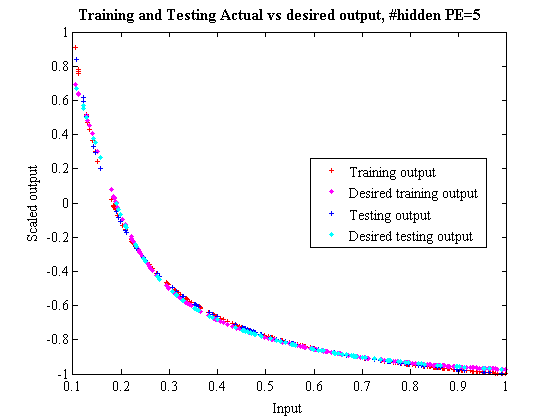
\includegraphics[width=4.5in]{PE5.png} }


We then compared the difference of error over time with different PEs. The comparison of error history over time is shown as figure below. The error curves have no peaks as shown in problem2, which indicates that the momentum helps converging. From this figure we can notice that the one with best fitting rate are hidden PE number being equal to 8 and equal to 5. However, the best hidden PE number is not the same all the time (data not shown), revealing the fluctuation of learning.



	\centerline{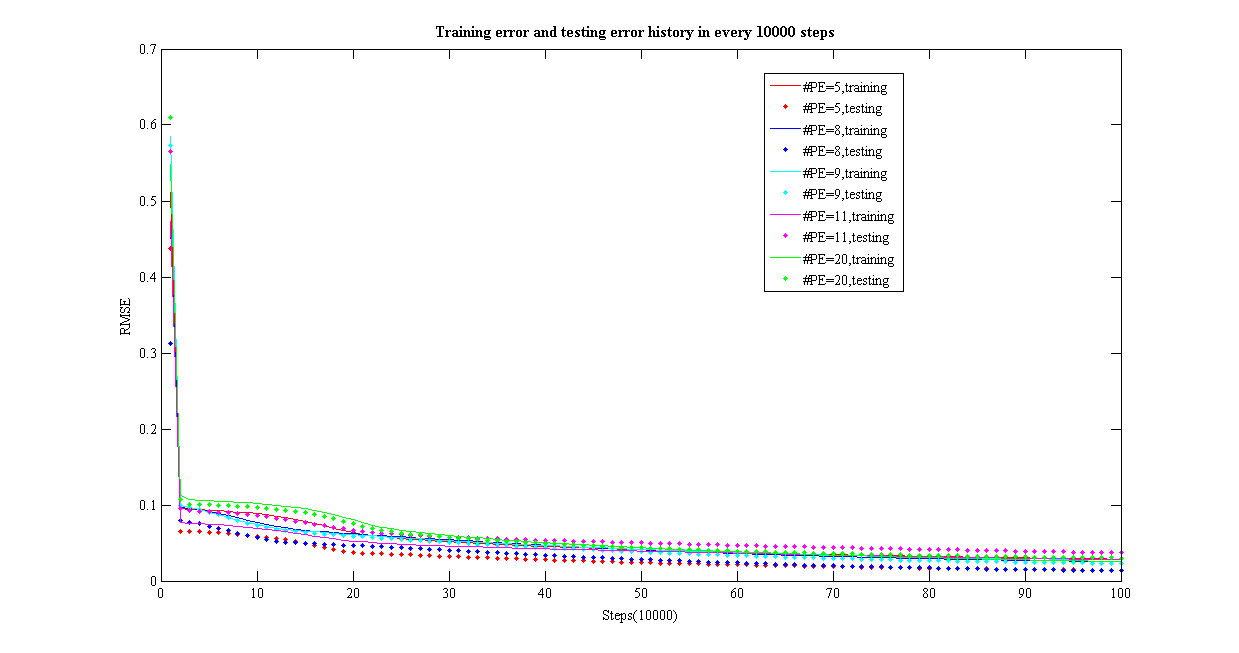
\includegraphics[width=6.5in]{errhistory.png} }


\clearpage

{\bf 
	\npar
	b Different momentum
	\bpar
}

We hoped to further understand the function of momentum and we tested several of them. Since the testing result showed that the recalling and generalizing were successful (the outputs are similar, while there can be some difference in error rate), we here then only show the testing data.

\begin{table}[htbp] 
	\center
	\caption{Parameters of Training BP Network to Fit $f(x) = 1/x$ with different momentum}

	%\scalebox{0.9}{ % You can scale the size of the table by changing this number
	\scalebox{1.0}{
		\begin{tabular}{p{4cm} p{.05cm} p{8cm}}
			\toprule
			\multicolumn{3}{l}{\bf Network parameters} \\
			\bottomrule \noalign{\smallskip}
			Topology & & $(1 + 1_{Bias})$ --- $8+1_{Bias}$ --- 1 \\
			\toprule
			\multicolumn{3}{l}{\bf Learning parameters} \\
			\bottomrule \noalign{\smallskip}
			Learning rate ($\alpha$) & & 0.006\\
			Momentum & &  0.2, 0.4, 0.6, 0.8 \\
			
			\bottomrule \noalign{\smallskip}
		\end{tabular}
	} % end scalebox
\end{table}

The figure below reveals the output using different momentum. we can see that when momentum get to 0.8, it is too large to make the result converge to a desired error rate.


	\centerline{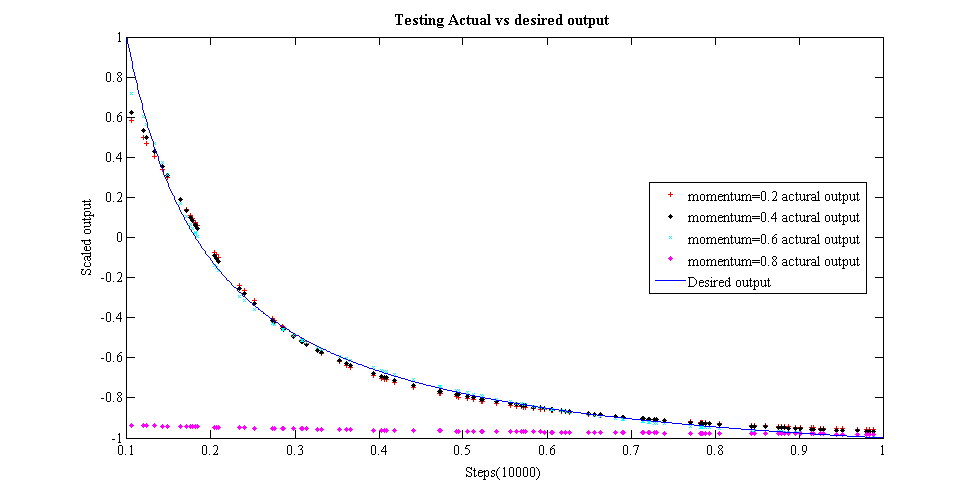
\includegraphics[width=6.5in]{momentum_output.png}} 


Also, the error rate history of testing set using different momentum are shown in the figure below. When momentum is around 0.6, the final error rate becomes the lowest.


	\centerline{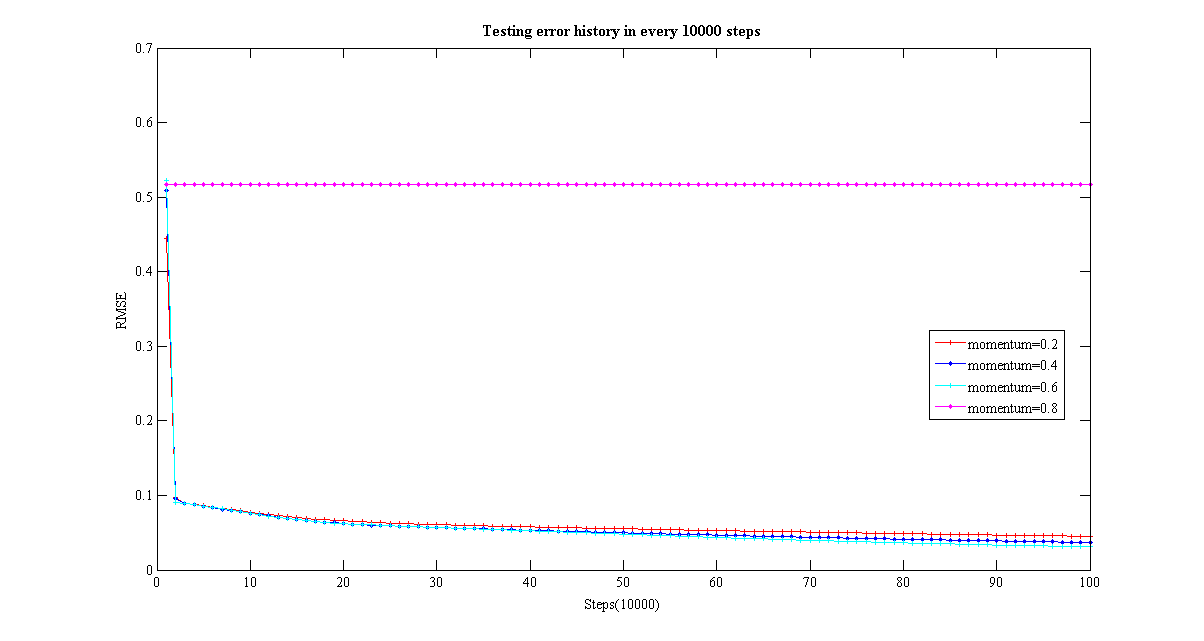
\includegraphics[width=6.5in]{momentum_error.png}} 


\clearpage

{\bf 
	\npar
	c The best results
	\bpar
}

From all the figures above we can find that, though finally the reducing of error was getting to a plateau stage, we can still have lower error rate with more steps. Here we limit the maximum learning step as 1,000,000, which is the same as shown before. 


\begin{table}[htbp] 
	\centering
	\caption{Parameters of Training BP Network to Fit $f(x) = 1/x$ that gives the best results}

	%\scalebox{0.9}{ % You can scale the size of the table by changing this number
	\scalebox{1.0}{
		\begin{tabular}{p{2cm} p{3cm} p{2cm}p{2cm} p{2.5cm}}
			\\\toprule
			\multicolumn{5}{l}{\bf Network parameters} \\
			\bottomrule \noalign{\smallskip}
			Topology &$(1 + 1_{Bias})$ --- & $8+1_{Bias}$ & --- 1 &  \\
			\\\toprule
			\multicolumn{5}{l}{\bf Learning parameters} \\
			\bottomrule \noalign{\smallskip}
			&Learning rate ($\alpha$)  &  Momentum & Testing error &  Training error\\
			Set 1 &0.006 &  0.68& 0.0151  & 0.0261 \\
			Set 2 &0.01 & 0.1 & 0.0289  & 0.0392 \\
			Set 3 &0.015 & 0.3 & 0.0145  & 0.0219 \\
			\bottomrule \noalign{\smallskip}
		\end{tabular}
}
\end{table}



The three best outputs are shown in the figure below. Here we only showed the testing output since the training outputs are similar to them in this graph. We can also notice that when input get to a larger value, the learning and the regression is better.



	\centerline{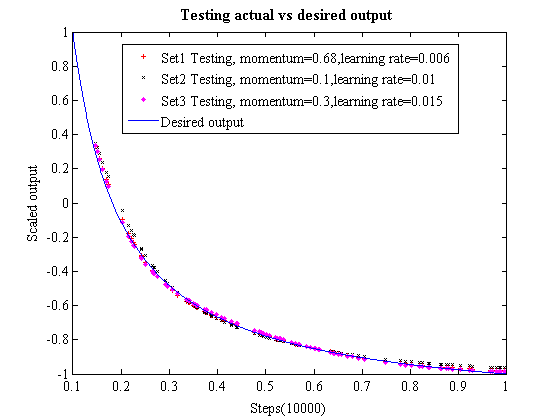
\includegraphics[width=6in]{best_output.png} }


Also, we showed the history of error rate reduction over time. 

	\centerline{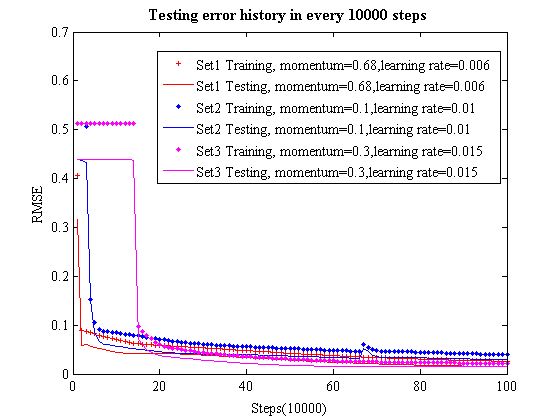
\includegraphics[width=6.5in]{best_err.png} }


\clearpage

{\bf 
\npar
Problem 4
\bpar
}

\begin{table}[htbp] 
\center
\caption{Parameters of Training BP Network to Fit Iris data}

  %\scalebox{0.9}{ % You can scale the size of the table by changing this number
   \scalebox{1.0}{
   \begin{tabular}{p{4cm} p{.05cm} p{8cm}}
\toprule
  \multicolumn{3}{l}{\bf Network parameters} \\
\bottomrule \noalign{\smallskip}
  Topology & & $(4 + 1_{Bias})$ --- $(2+1_{Bias} )$ --- $3$ \\
  Transfer function & & tanh with slope of 1 \\
\toprule
  \multicolumn{3}{l}{\bf Learning parameters} \\
\bottomrule \noalign{\smallskip}
  Initial weights & & drawn from U[$-1\over{\sqrt{NPE}}$,$1\over{\sqrt{NPE}}$] \\
  Learning rate ($\alpha$) & & 0.01 \\
  Momentum & & 0.7\\
  Epoch size ($Epoch$)& &  75 \\
  Stopping criteria & & RMSE$ < 0.2$ or  learn count (t) $ > 500 \times 75 $\\
  Error measure & &$1-{{Number\ of\ CorrectlyClassified\ Inputs}\over{Number \ of\ All\ Inputs}}$(1-Accurancy) and RMSE \\\toprule
 \multicolumn{3}{l}{\bf Input / output data, representation, scaling} \\
\bottomrule \noalign{\smallskip}
  \# training samples ($N_{tr}$)& & 75 \\
  \# test samples ($N_{tst}$)& & 75 \\
  Scaling of inputs & &  already scaled \\
  Scaling of outputs & &  set the maximum element of each column to 1, others to 0  \\

 \bottomrule \noalign{\smallskip}
 
  \end{tabular}
   } % end scalebox
\end{table}
* As stated, we calculate the error using scaled output, so "Correctly Classified" means exactly same output as desired.\\
\centerline{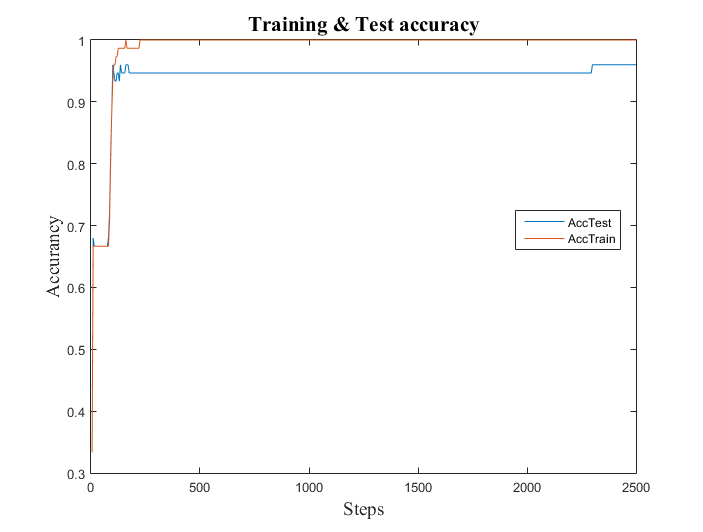
\includegraphics[width=4in]{p41.png}} 
\centerline{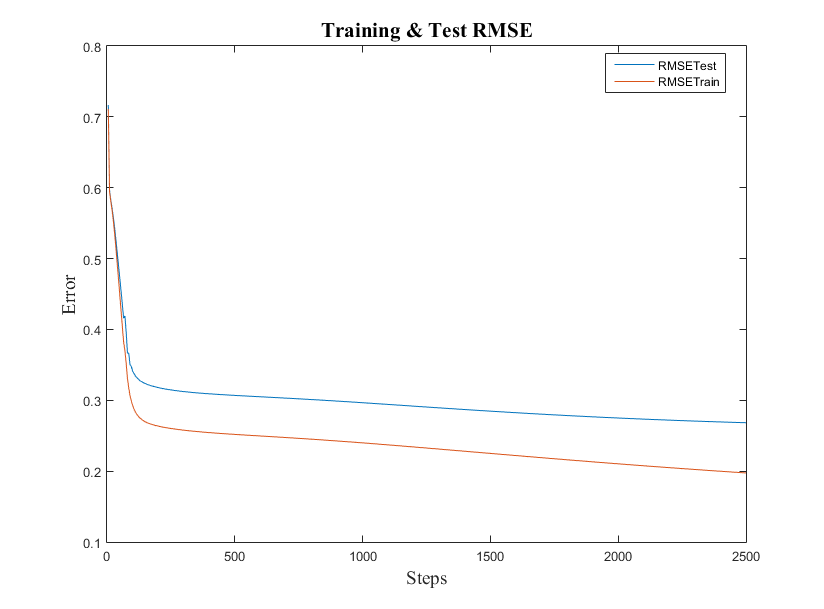
\includegraphics[width=4in]{p42.png}} 
		

			
		\begin{table*}[htbp]
			\centering
			\caption{Desired output vs Actual output(Test set)}
			\begin{tabular}{|l|ccc|}
				
				\hline
				
				\diagbox{Actual}{Desired} & Class 1 & Class 2 & Class 3 \\
				\hline
				Class 1&25 &0 &0\\
				Class 2&0 & 24&2\\
				Class 3&0 &1 &23\\
				\hline
				Accurancy &1&0.96 & 0.92\\
				\hline
			\end{tabular}\\
			Total Accurancy:0.96\\
			\spar
			*Class 1 is Setosa, Class 2 is Versacolor, Class 3 is Virginica
		\end{table*}

		
In this problem, we tried different topology and training parameters. We find it needs at least 2 hidden PEs to get good result, and more hidden PEs cannot improve the performance. We also tried different momentums and learning rates. As expected, we find that large momentums or learning rate will make the training doesn't converge. Furthermore, smaller learning rate/momentum or more training iterations cannot increase the accurancy. So we pick the largest learning rate and momentum(among we tested) to achieve fastest convergence.\\
\spar
As stated in the parameter table, this time we use RMSE rather than  classification error as the stopping criteria. When we plot the change of Accurancy and RMSE along triaining iterations, we can see that even the Accurancy of trianing set hit 100\%, the RMSE of both test and training set is still decreasing, and the Accurancy of test set increases after 2,000 learning steps. So if we use the accurancy as the stopping criteria, it will limit the performance of the network.\\
\spar
We think for small datasets as this time, use RMSE as stopping criteria could give better result. Maybe if the dataset is large, restrict the classification accurancy could prevent overfitting issues.\\
\spar
We gives the "Desired output versus Actual output" plot as a classification matrix(Table 7). It's straightforward and contains all the informations we concerned: the performance of each class and the location of error(Since no one concerns the order of samples). Since the training set is perfectly classificated, we didn't show the results for training set.\\
\spar
From Table 7 we can see only class 1 is perfectly classified. Maybe its because class 1 is linearly seperatable from the other 2 classes.
 
\end{document}